\documentclass[runningheads,a4paper,fleqn]{llncs}

\usepackage{url}
\usepackage{amsmath}
\usepackage{amssymb}
\usepackage{alltt}
\usepackage{lineno}
\usepackage{graphicx}
\usepackage{subfigure}
\usepackage[normalem]{ulem}

\usepackage{tikz}
\usetikzlibrary{arrows,petri,topaths}
\usepackage{tkz-berge}

\begin{document}

\title{FlowArrays: Barrier-Free ParArrays}
\author{Tobias Schlatter\inst{1} \and Aleksandar Prokopec\inst{2} \and
  Heather Miller\inst{2} \and Philipp Haller\inst{2} \and Martin
  Odersky\inst{2}}

\authorrunning{Tobias Schlatter}

\institute{Student, EPFL \and Advisors, EPFL}

\graphicspath{{figs/}}

\newcommand{\plot}[1]{\input{../../benchmarks/flowArrays/plots/#1}}

\maketitle

\begin{abstract}
  In \cite{FP12} we proposed an unordered, barrier- and lock-free,
  parallel datastructure, the FlowPools. The following attempts to
  implement a bigger application using FlowPools, showed that the lack
  of ordering is very limiting. The proposed FlowArrays do not have
  this limitation: Having a very similar structure than ParArrays
  \cite{collect11}, FlowArrays eliminate the need to block in between
  monadic operations on ParArrays while exposing a very similar
  interface to the programmer.

  Benchmarks on operations for linear algebra have shown that the
  current basic storage model of FlowArrays severely impacts
  performance and that the adaptions proposed later on in this report
  do significantly speed up the calculation but still need to be
  properly generalised.
\end{abstract}

\section{Introduction}
TODO This is the usual blah about nothing but which is
required... Parallel architectures are more and more important and the
need to have languages... 

We'll first give an overview of the general idea behind FlowArrays and
how they try to improve on ParArrays. In next section
(c.f. page~\pageref{sec:implementation}) we'll explain in more detail,
how FlowArrays are implemented. The evaluation section
(c.f. page~\pageref{sec:evaluation}) will analyse the performance of
FlowArrays using vector scalar products as benchmark. In the
conclusion (c.f. page~\pageref{sec:conclusion}), we'll propose
improvements and future work.

\section{Overview}
\label{sec:overview}

In this section we'll first outline how FlowArrays try to improve on
ParArrays from an abstract perspective. Then we'll show some of the
difficulties that arise particularly with this approach.

\subsection{Barrier-Freedom}
FlowArrays in comparison to ParArrays are barrier-free: We'll
illustrate on the simplest example, a single \texttt{map} map
operation, how these two datastructures differ.

Let's consider the following code for ParArrays and
FlowArrays. Fig.~\ref{fig:barrier-free} shows a schematic
illustration of what's going on.

\noindent
\begin{minipage}[t]{.5\textwidth}
\begin{alltt}
{\scriptsize
val pa1 = ParArray.tabulate(n)(x => x*x)
val pa2 = pa1.map(_ * 2)
}
\end{alltt}
\end{minipage}
\begin{minipage}[t]{.5\textwidth}
\begin{alltt}
{\scriptsize
val fa1 = FlowArray.tabulate(n)(x => x*x)
val fa2 = fa1.map(_ * 2)
}
\end{alltt}
\end{minipage}

In both cases, we first create a Par/FlowArray using a tabulate. Both
Par- and FlowArrays will use exponential task splitting
\cite{collect11,cong08} to distribute the workload of calculating the
individual elements. The crucial difference between ParArrays and
FlowArrays starts here: With ParArrays, the call to \texttt{tabulate}
(and any other function for that matter) will only return, once every
element has been calculated. In contrast, the call to
\texttt{tabulate} on FlowArrays will return immediately, yielding an
array whose elements are specified, but not yet calculated.

When calling \texttt{map} on the first Par/FlowArray, this difference
becomes even clearer: ParArrays will do the same thing as for
\texttt{tabulate}: Split up the task of calculation and start right
away. FlowArrays however, will align the task blocks and start
calculating the elements, once the elements the result depends on have
been calculated (in our case the result of the \texttt{tabulate}). So
contrary to ParArrays, FlowArrays are able to start subsequent
calculations partially, even if not all the elements of the original
array have been calculated.

\begin{figure}
  \centering
  \subfigure[ParArray] {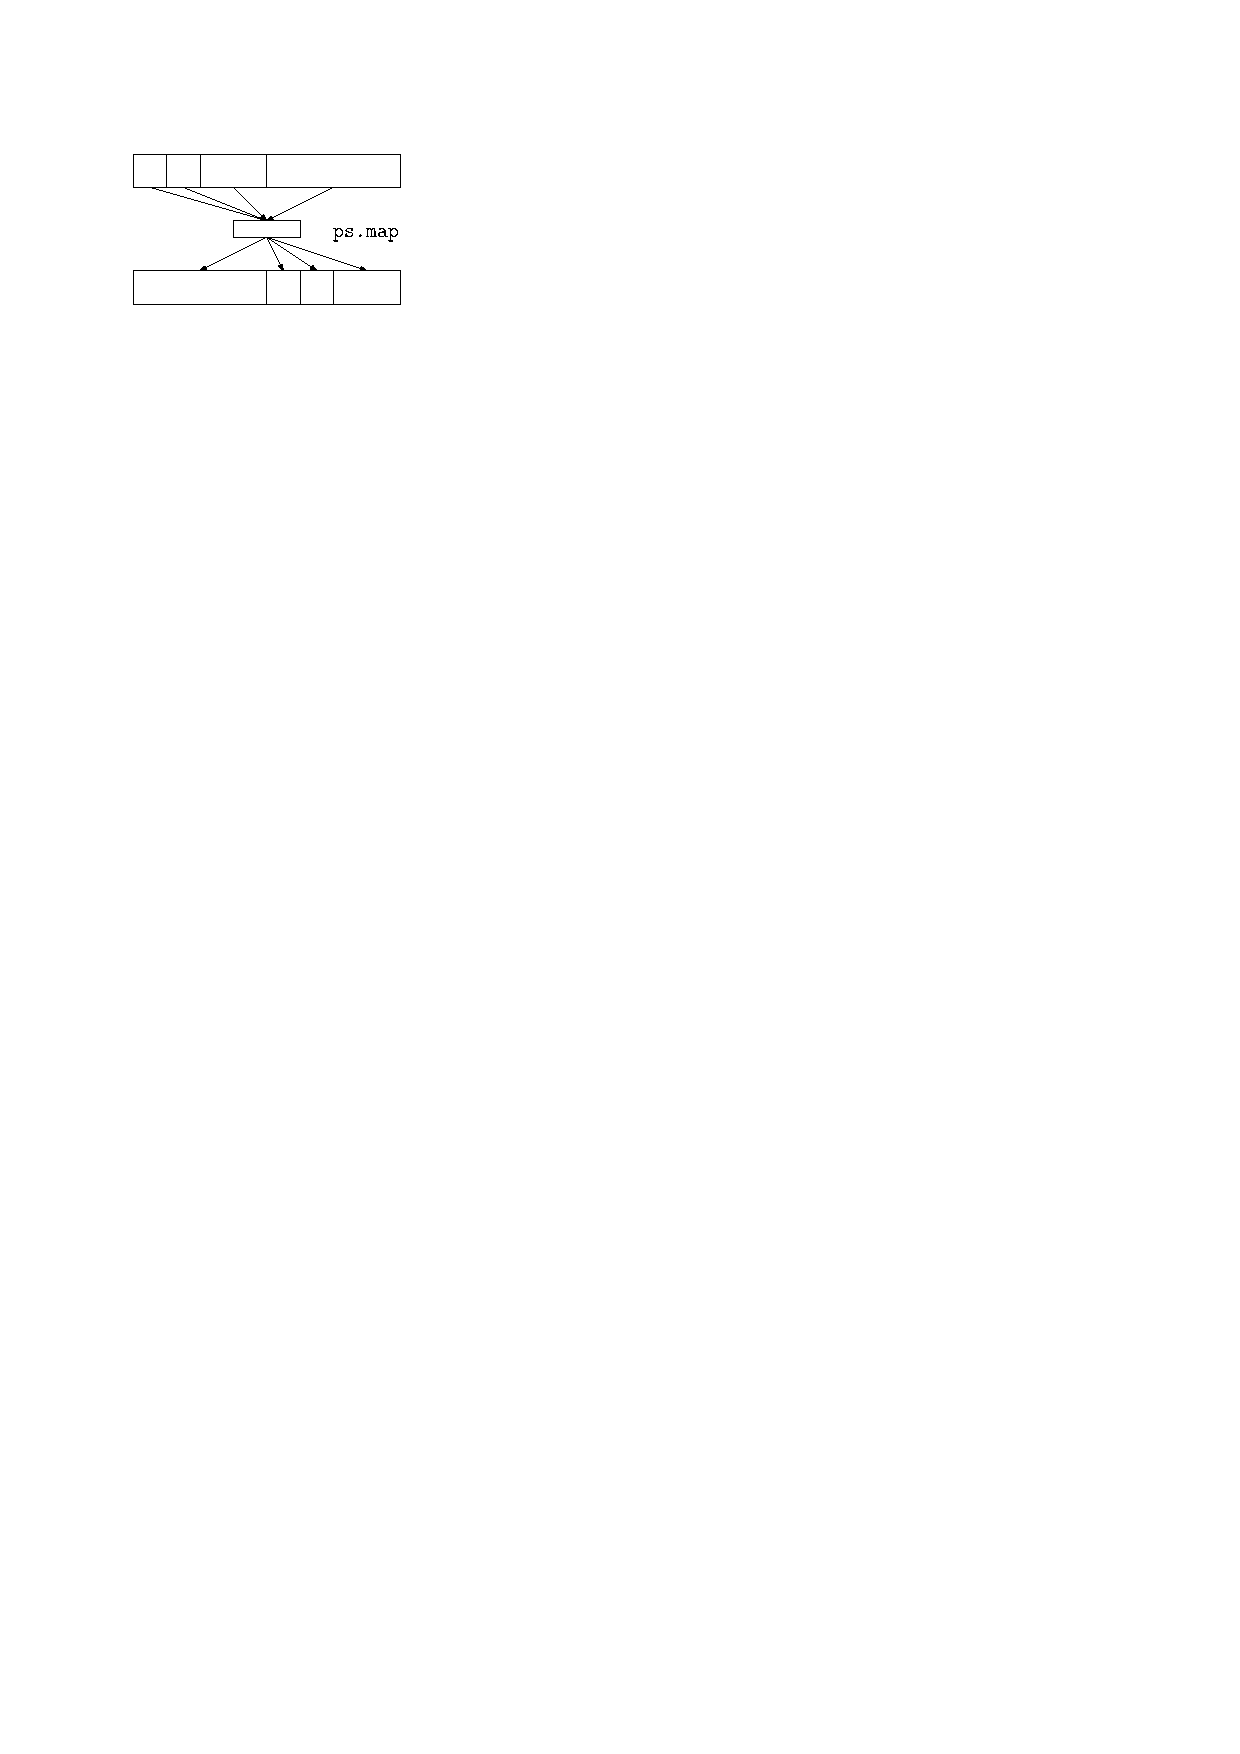
\includegraphics{barrier-free-pa}}
  \qquad
  \subfigure[FlowArray]{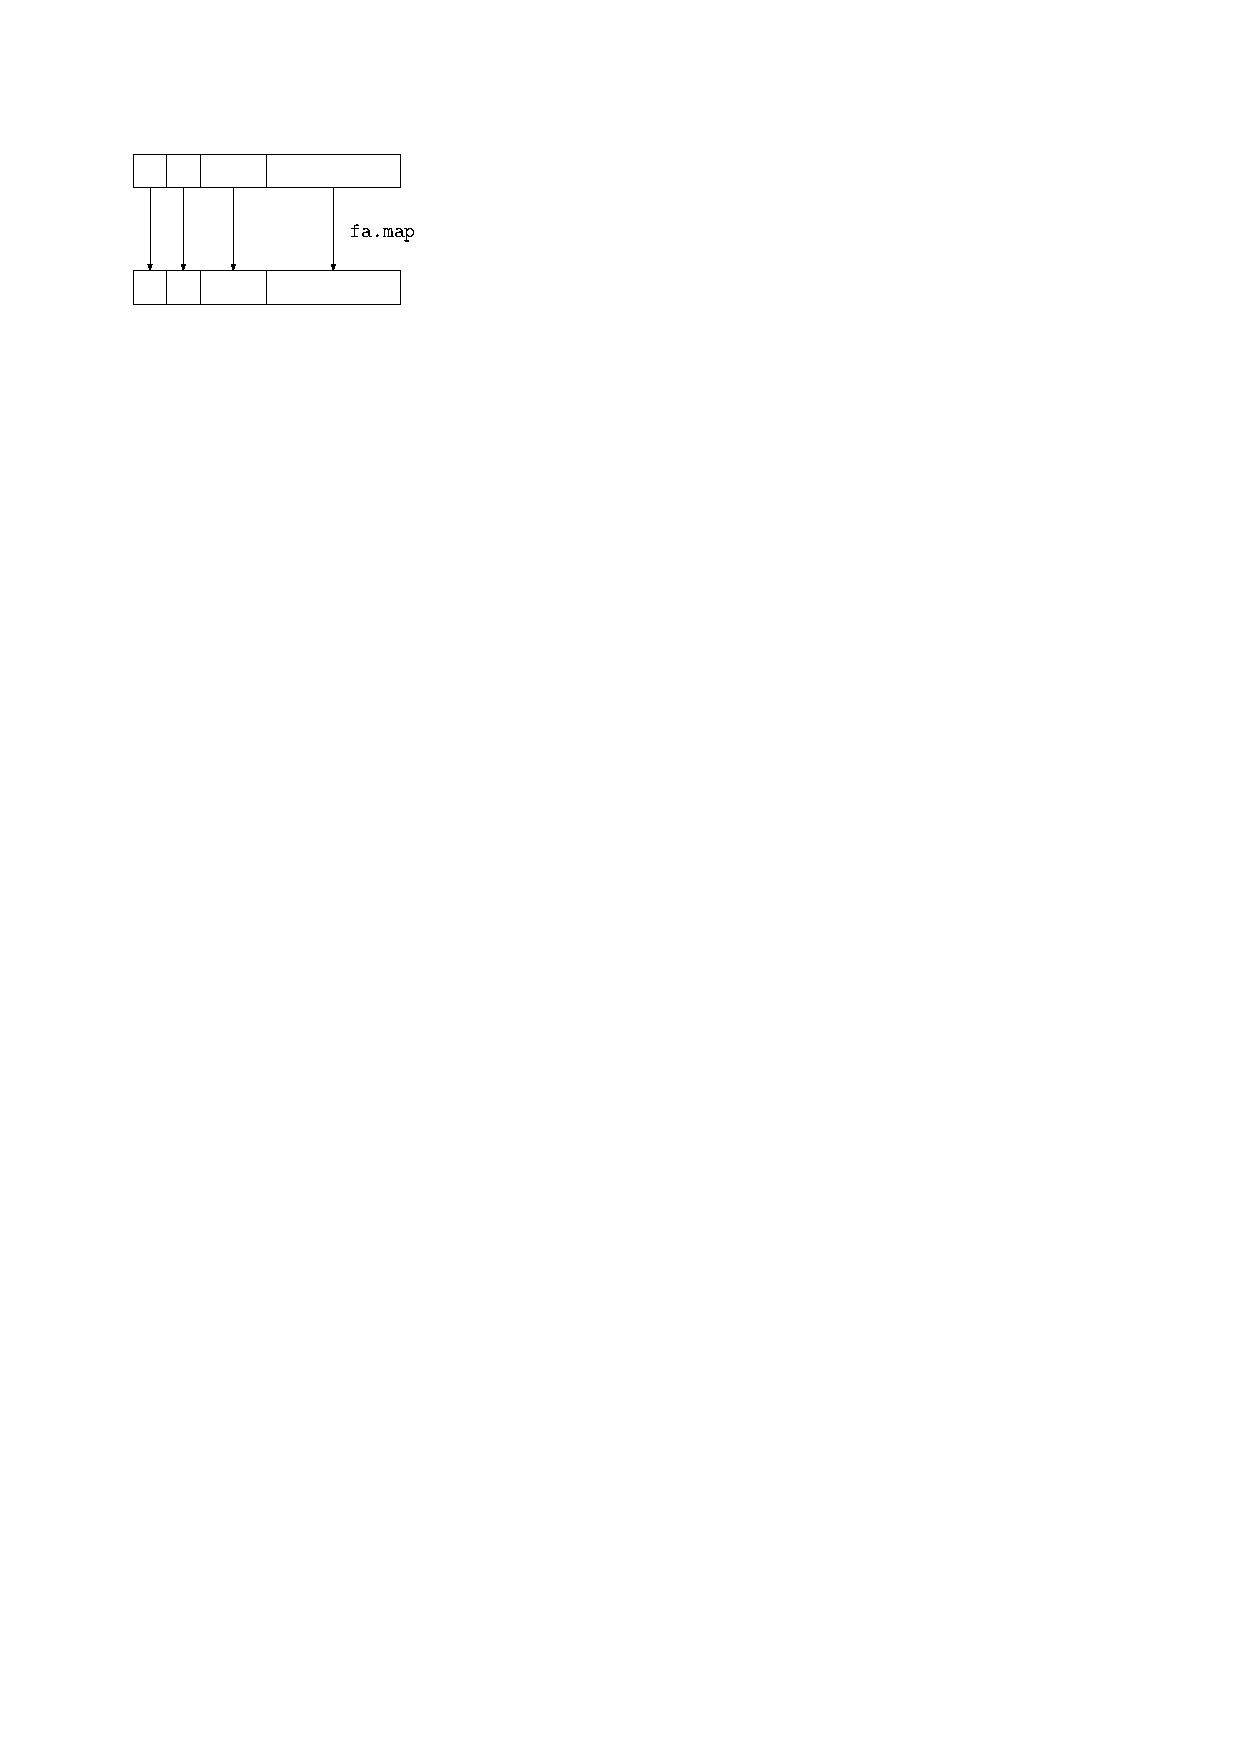
\includegraphics{barrier-free-fa}}
  \caption{Illustration of barrier-freedom of FlowArrays}
  \label{fig:barrier-free}
\end{figure}

\subsection{Dependency Tracking}
We'll now describe in detail what happens, when a \texttt{map} is
called on a FlowArray depending on the different possible states of
its blocks. Fig~\ref{fig:dep-track} illustrates the different
scenarios that may happen. In the figure, the circles represent jobs:
grey if executing or submitted to the execution queue, white if
waiting in an internal queue of another job (indicated by the dashed
arrow). The rectangles represent data blocks of a FlowArray: white if
(partially) empty, grey if fully calculated.

When a \texttt{map} is called on a FlowArray, each block chain will
start in one of the three first states and then propagate to the right
until both blocks are fully calculated. The cases are the following:

\begin{figure}
  \centering
  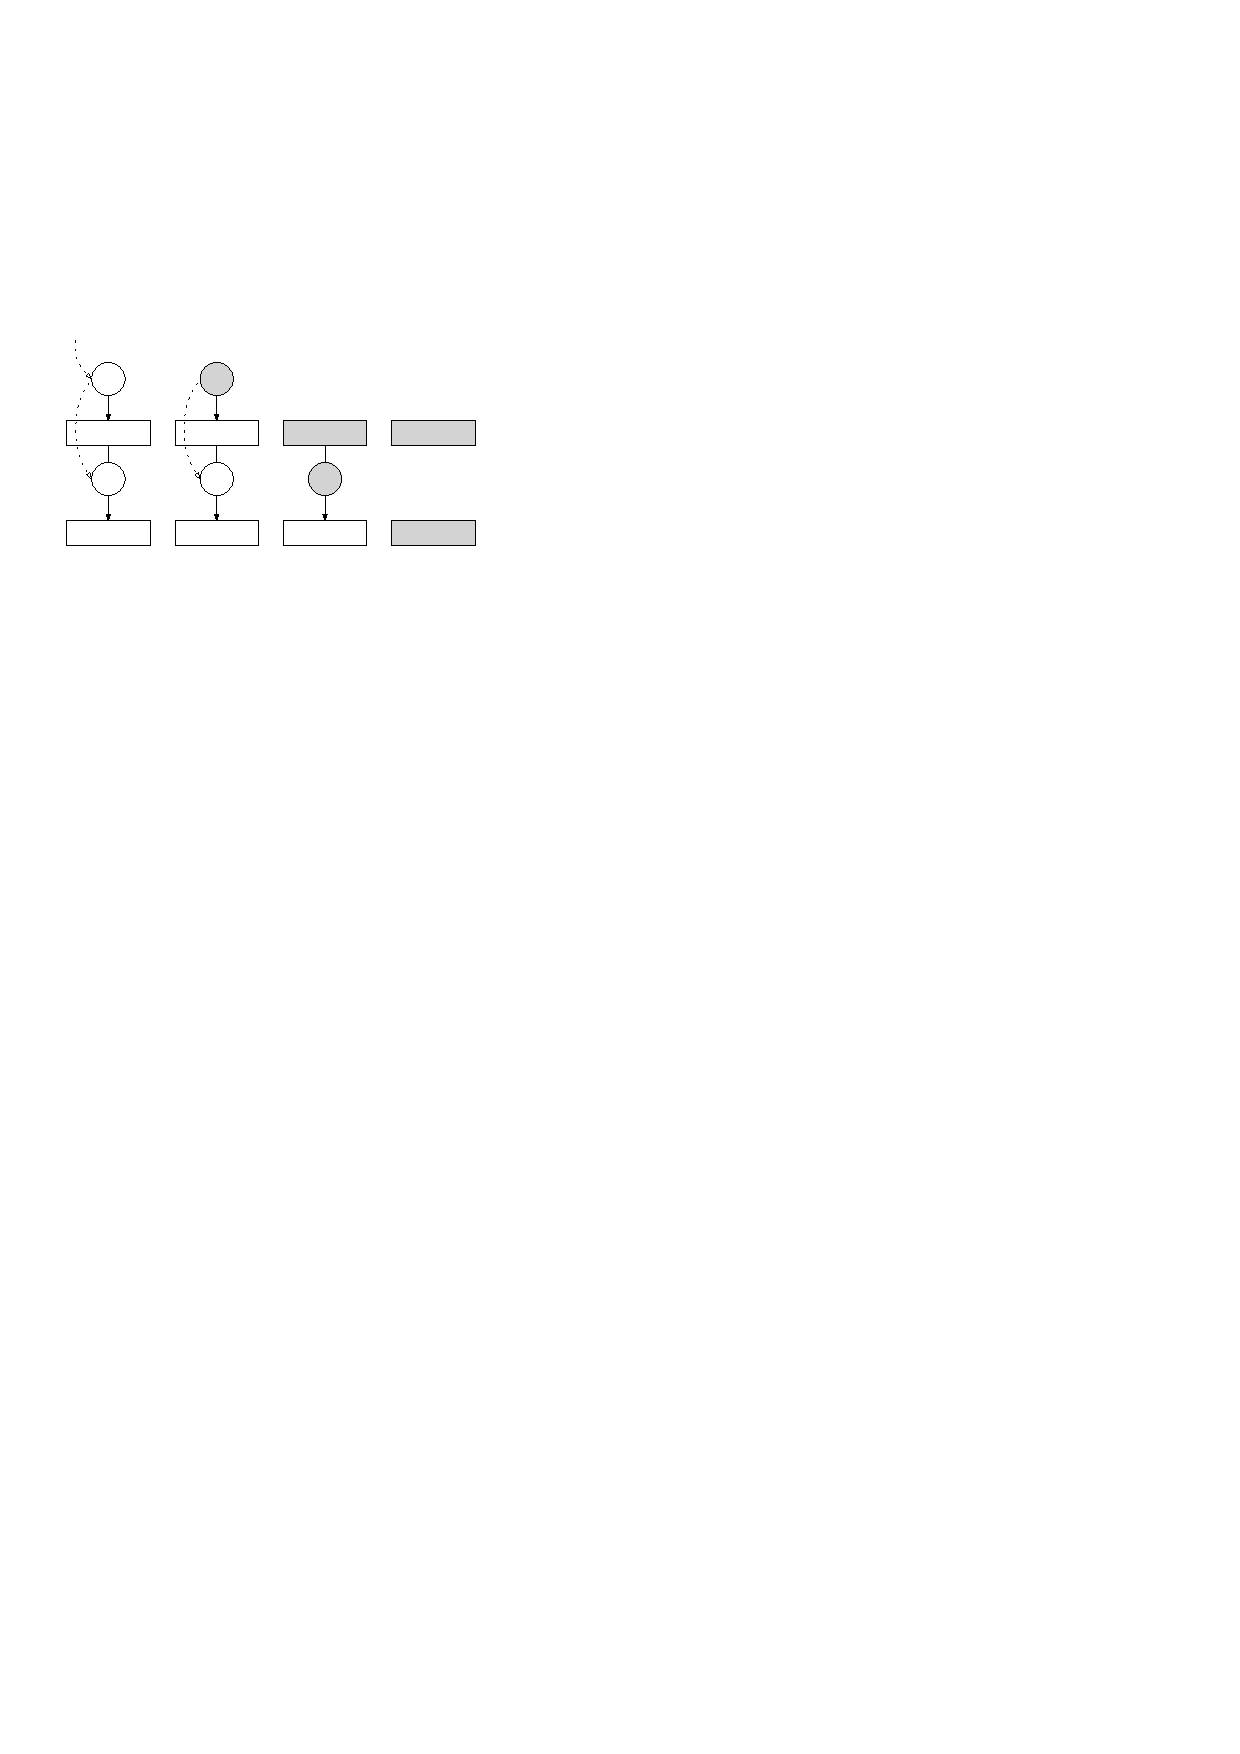
\includegraphics{dependency-tracking}
  \caption{Illustration of the dependency tracking in FlowArrays}
  \label{fig:dep-track}
\end{figure}


\begin{enumerate}
\item Both blocks are not yet calculated and the job for the first
  block still depends on some other job: The second job is added to
  the first job's dependency queue.
\item The job for the first block is scheduled for execution but not
  yet finished: The second job is added to the first job's dependency
  queue.
\item Calculation of the first block is already completed: The second
  job is scheduled for execution immediately.
\item Both blocks are completely calculated.
\end{enumerate}

\subsection{Operations}
We have seen how dataflow with dependency tracking can be used in
monadic operations on the example of a \texttt{map}. In this section
we'll describe the caveats of other common monadic operations on
arrays.

\subsubsection{Fold}
When doing out of order folding, each block has first to be reduced to
a single element, then these results have to be combined to the final
result. During splitting of the jobs, one can create a binary tree of
blocks along which one can later accumulate the elements;
fig~\ref{fig:fa-fold} illustrates this approach.

\begin{figure}
  \centering
  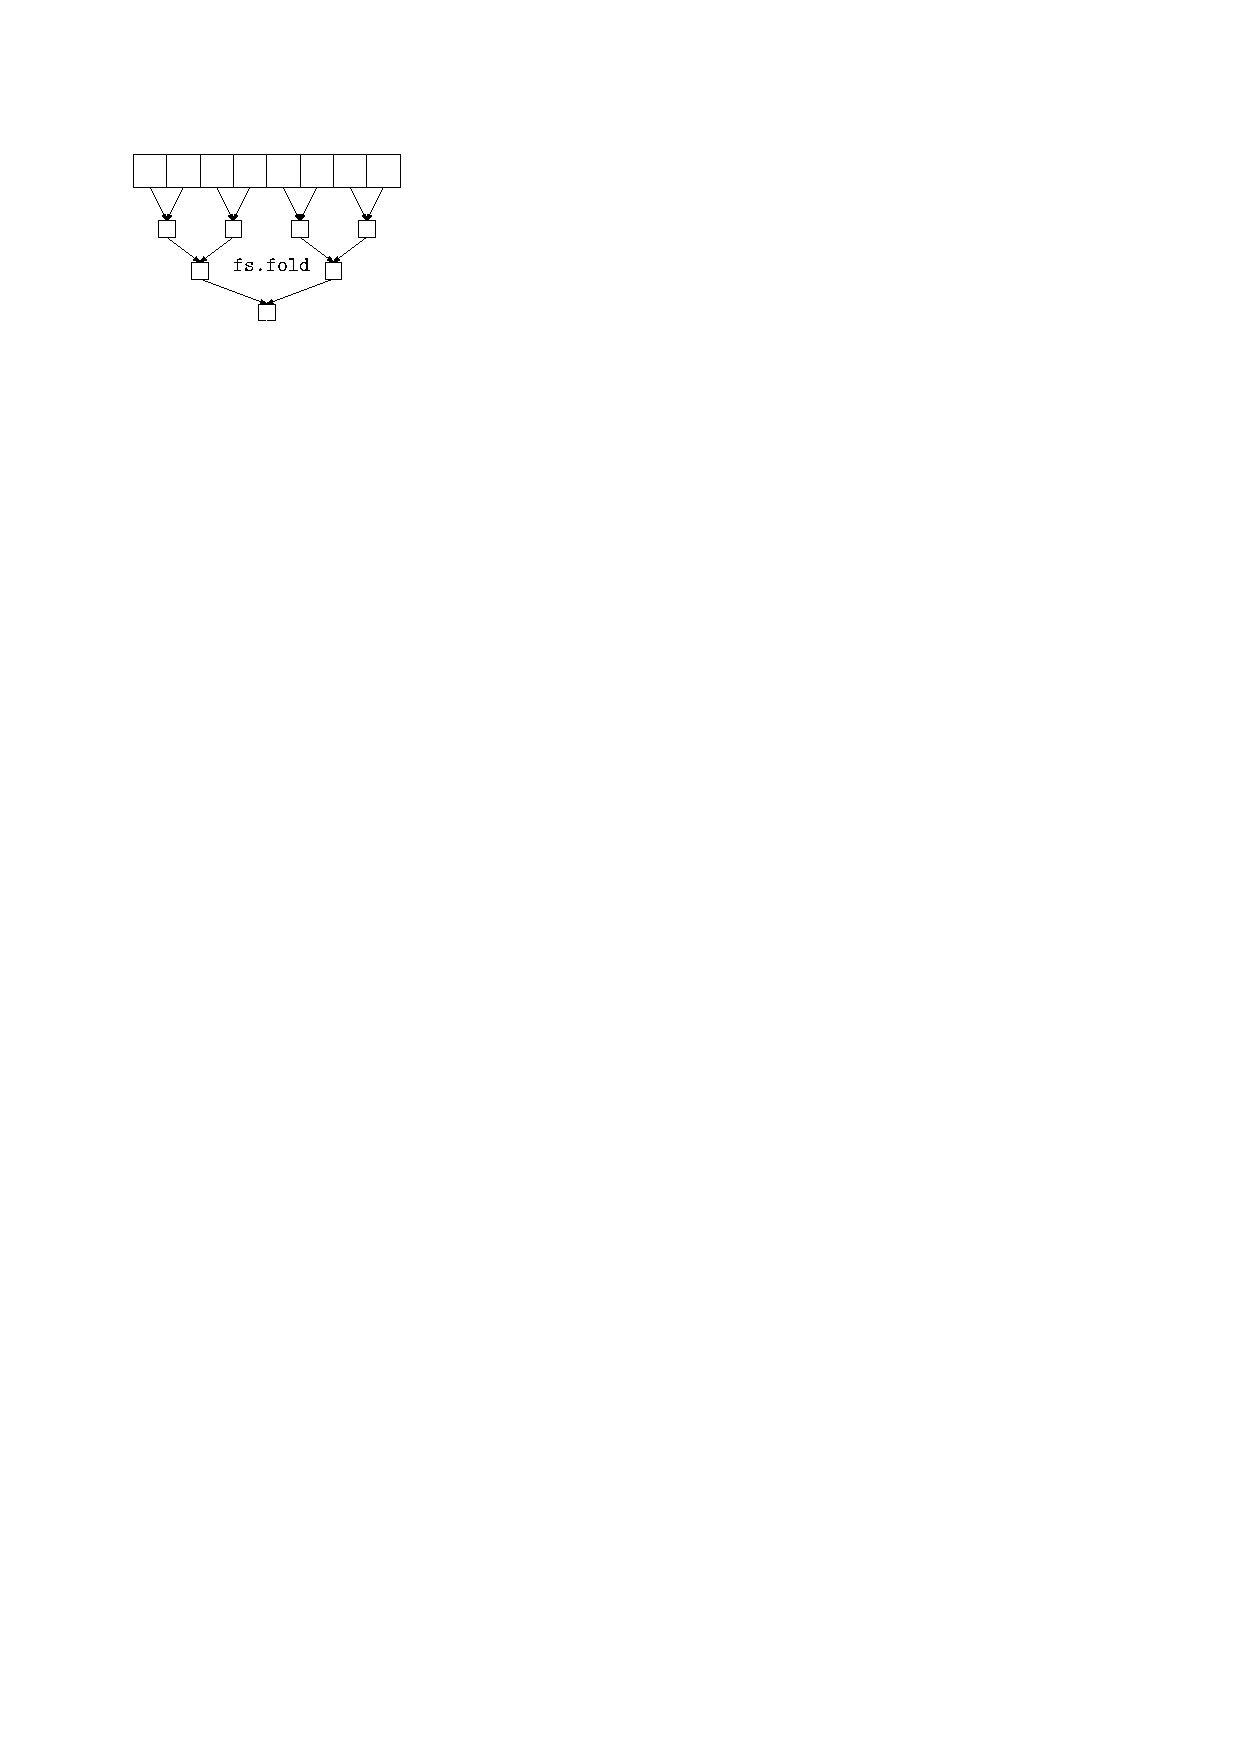
\includegraphics{fa-fold}
  \caption{Illustration of \texttt{fold} on a FlowArray}
  \label{fig:fa-fold}
\end{figure}

In order to keep the number of jobs (and hence the burden of managing
them) minimal, rather then spawning a single job for each accumulation
step in the tree, the job which finishes second on each node is
responsible to calculate its accumulated value. Using this scheme, the
same number of jobs are spawned as for a \texttt{map}.

Note that this approach is preferable to a single element where
completed elements are accumulated using a CAS since the former
does preserve the order in which elements are accumulated. I.e. it
requires the accumulation function to be associative, not
commutative.

\subsubsection{FlatMap}
\label{sssec:flatMapN}

When calling flatMap on a FlowArray, the size of the resulting
FlowArray is not known until the inner FlowArrays are created and
hence their size can be read. However, since this happens
asynchronously, the size of the resulting FlowArray would not be known
at its creation. This poses several challenges:

\begin{itemize}
\item The interface of FlowArrays becomes more complex
\item Increased difficulty in memory allocation
\item Increased difficulty in scheduling of subsequent calls
\end{itemize}

Instead of deferring the size calculation, FlowArrays require to pass
the size of the resulting FlowArrays of a \texttt{flatMap} operation
when calling it (therefore the name \texttt{flatMapN}). This greatly 
facilitates further handling -- especially scheduling -- of the
resulting FlowArray.

Further, the FlowArray now needs to keep track of dependencies twice:
Once, whether a sub-FlowArray has already been created, second,
whether a given one of its blocks is already calculated. Refer to
fig~\ref{fig:flatMap-dependency} for an illustration. This tracking
requires the outer FlowArray to keep references to all the created
ones. In order to avoid unnecessary copying of data, the FlowArray
remains in this hierarchical structure instead of being truly
flattened.

\begin{figure}
  \centering
  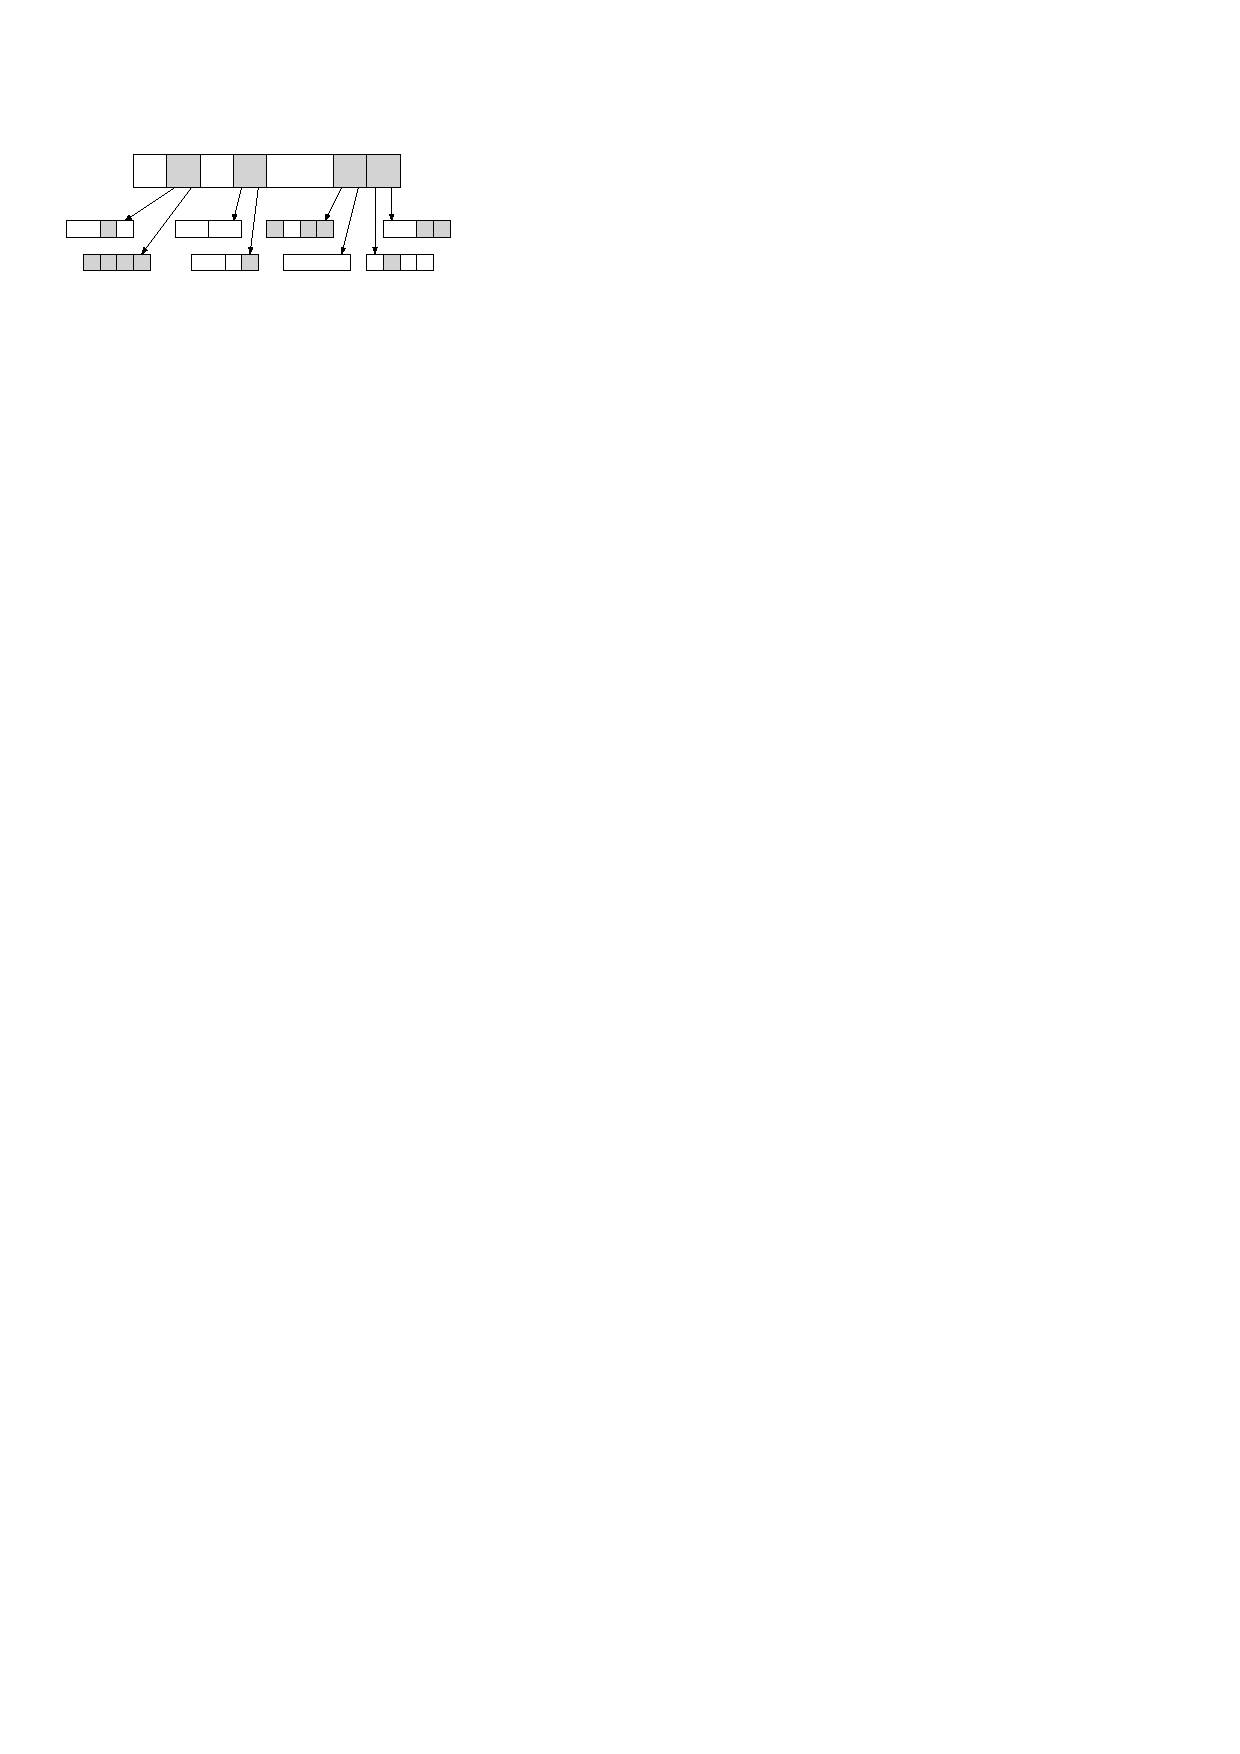
\includegraphics{flatMap-dependency}
  \caption{Illustration of dependency-tracking requirements in a
    Hierarchical FlowArray resulting from a \texttt{flatMap}}
  \label{fig:flatMap-dependency}
\end{figure}

When a \texttt{map} is called on one of these \emph{Hierarchical
  FlowArrays} individual \texttt{maps} are called for each sub array
and only then the resulting data is written in a flat array. This
allows to ``flatten out'' those hierarchical structures without
additional computation costs. Note that this scheme does require the
blocks to be re-aligned at a later point in time to remove the
arbitrary splitting imposed by the hierarchy introduced by the
\texttt{flatMap}. For details how block splitting is propagated
through dependencies, please refer to
section~\ref{sec:implementation}.

\subsubsection{Zip}
When zipping, again we impose a restriction on the size: the size of
the two FlowArrays which are being zipped need to be of the same
size. This is again to ease scheduling and implementation. However, in
this case, minor changes in the implementation could easily remove
this limitation (unlike \texttt{flatMap}, where the interface would
need to undergo a fundamental change).

Further, the splitting of the two FlowArrays which are being zipped
may be totally different, e.g. due to a preceding \texttt{flatMap} on
one of them. Hence -- again -- re-alignment of blocks is required,
before the zipped tuples can be created. It is important to realise,
that this may inherently lead to non-symmetric scheduling behaviour:
Depending on which FlowArray is on the ``left'' of the \texttt{zip}
call, the resulting splitting may be different, which may lead to
different speed at runtime. 

\section{Implementation}
\label{sec:implementation}

This section describes in some more detail, how the requirements
explained in section~\ref{sec:overview} are implemented. Note that
this is a simplified view and some interfaces may not be described
with all methods or all arguments of the methods. Further, methods may
be simplified (e.g. not tail-recursive for easier
understanding). Please refer to scaladoc for an API documentation.

\subsection{FlowArray Jobs}
The class \texttt{FAJob} is the heart-piece of the whole FlowArray
implementation: It handles computation, task splitting and dependency
tracking. An \texttt{FAJob} has a range it operates on
(\texttt{start,end}) and an abstract method that does the computation
(\texttt{doCompute}). Further, the following methods are supported for
dependency tracking, splitting and scheduling:

\begin{description}
  \item[\texttt{depending(newJob: FAJob): Unit}] Submits another \texttt{FAJob} as being
    dependent on this \texttt{FAJob}. This will schedule the submitted
    \texttt{FAJob}, once this \texttt{FAJob} is completed.
  \item[\texttt{split(): Unit}] Splits this job into two
    sub jobs. Forces dependent tasks to be split too and hands off
    dependency (see next section for details on splitting). This
    method is called when computation of a \texttt{FAJob} starts and
    its size is above the threshold for exponential splitting.
  \item[\texttt{done: Boolean}] Checks whether this \texttt{FAJob} is
    done. Queries sub jobs if this \texttt{FAJob} is split.
  \item[\texttt{sliceJobs(from: Int, to: Int): Option[(Seq[FAJob],
      Boolean)]}] Returns the jobs which are responsible for
    calculating a given slice. May require the caller to check again,
    once the jobs are completed (indicated by the Boolean flag). If
    the slice is completed, \texttt{None} is returned.
  \item[\texttt{delegateThen(d: Seq[FAJob])(thn: () => Unit): Unit}]
    This method may be called from inside the \texttt{doCompute}
    method only. It halts calculation of this \texttt{FAJob}, until
    all jobs in \texttt{d} are completed. It then (optionally)
    executes the closure \texttt{thn}.
\end{description}

\subsubsection{Splitting}
First
When calling \texttt{split} on a \texttt{FAJob}, two things have to be
done:
\begin{enumerate}
\item Split the job in two smaller sub jobs of (more or less) equal
  size.
\item Split the dependent jobs and delegate the dependency to the
  sub jobs: We would like to have dependency tracking on the lowest
  level that calculation is done in order to start new jobs as soon as
  possible (otherwise we'll be back at ParArrays).
\end{enumerate}

The first is easy: Divide the range of the \texttt{FAJob} into two
(more or less) equal ranges and create two new \texttt{FAJobs} with
those ranges.

The second is a bit more tricky. Please refer to fig~\ref{fig:split-ill}
for an illustration of how this is done. You find pseudocode in
fig~\ref{fig:split-code}. The idea is the following: First, create the
two sub jobs and set the state of this \texttt{FAJob} to
\texttt{Splitting}. It is now ``locked'' for any other operation. I.e. any
other operation must help the splitting first (as the implementation
is lock-free). Next, the dependent job must be split
(recursively). Once this is done, the dependants of the sub jobs may be
set to these newly created sub jobs. Finally the state of this
\texttt{FAJob} may be set to \texttt{Split}.

\begin{figure}
  \centering
  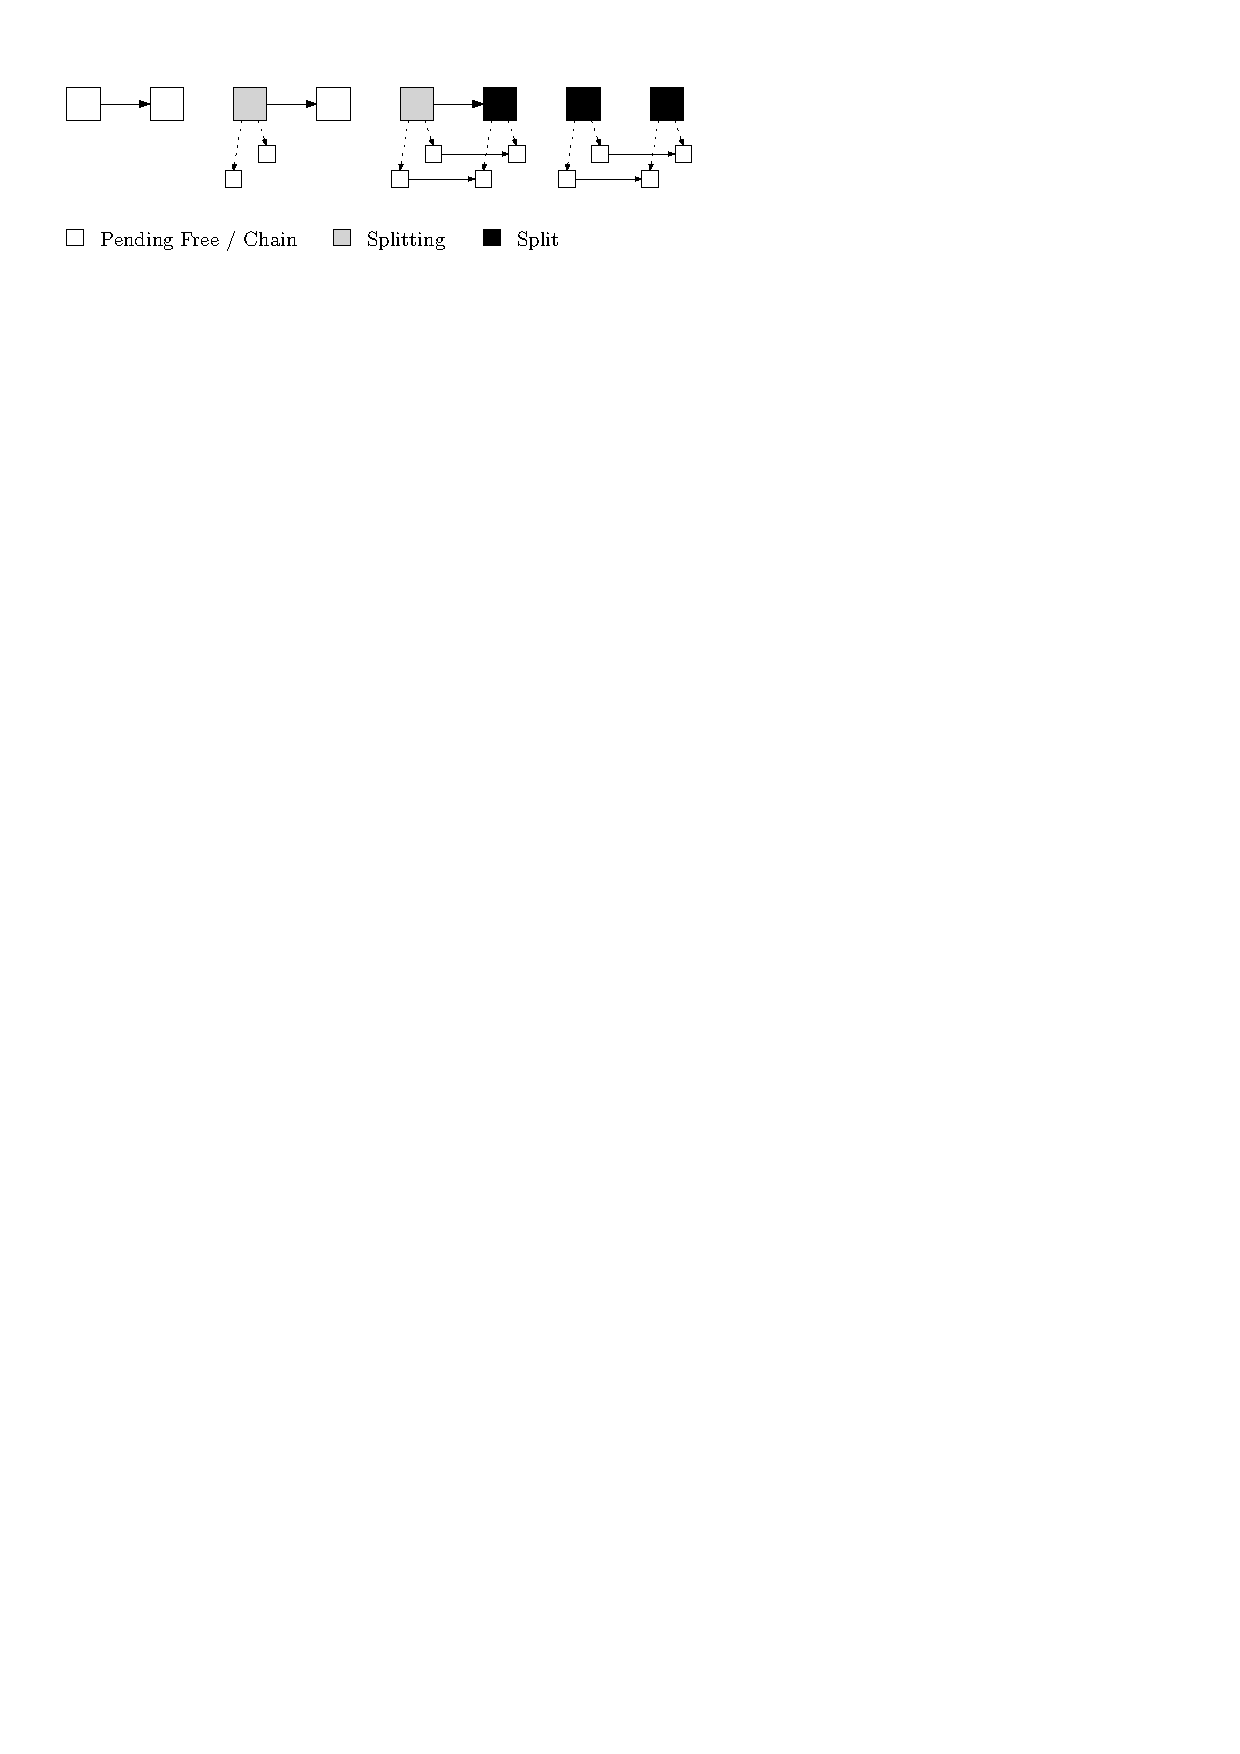
\includegraphics{split}
  \caption{Step-by-step illustration of splitting with dependencies}
  \label{fig:split-ill}
\end{figure}

\begin{figure}
\begin{minipage}[t]{7cm}
\begin{alltt}
{\scriptsize
def split(): (FAJob, FAJob) = state match \{
  case os@PendingFree =>
    val sj = newSubJobs
    if (CAS(state, os, Split(sj))) sj
    else split()
  case os@PendingChain(nextJob) =>
    val sj = newSubJobs
    CAS(state, os, Splitting(sj, nextJob))
    split()
  case os@Splitting(j1, j2, nextJob) =>
    val (nj1, nj2) = nextJob.split()
    j1.setNext(nj1); j2.setNext(nj2)
    CAS(state, os, Split(j1, j2))
    (j1, j2)
  case Split(j1, j2) => (j1, j2)
  case _ => error("Job already started")
\}
}
\end{alltt}
\end{minipage}
\begin{minipage}[t]{4cm}
\begin{alltt}
{\scriptsize
def compute() \{
  if (needSplit) \{
    val (j1, j2) = split()
    invokeAll(j1, j2)
  \} else \{
    doCompute()
  \}
\}
}
\end{alltt}
\end{minipage}
\caption{Pseudo-code for splitting and how splitting is invoked upon
  computation}
\label{fig:split-code}
\end{figure}

\subsection{FlowArray}
FlowArrays are the trait exposed to the API user. They (currently)
support the following common monadic operations \texttt{map},
\texttt{fold}, \texttt{flatMapN}\footnote{See
  section~\ref{sssec:flatMapN} on why the \texttt{N} in
  \texttt{flatMapN}}, \texttt{zip}, \texttt{slice}, \texttt{flatten}
and the generator \texttt{tabulate}.

Further, the a bit strange operation \texttt{transpose} is supported
to allow for matrix multiplication. For a more detailed view on
certain operations, have a look at
section~\ref{ssec:imp-operations}. Throughout the following sections,
the operation \texttt{map} is used as an example.

Internally two major types exist: \texttt{ConcreteFlowArrays} and
Views. \texttt{ConcreteFlowArrays} store actual data -- the most
trivial being the \texttt{FlatFlowArray}, which just wraps around an
Array. Views on the other hand expose data from
\texttt{ConcreteFlowArrays} under a different form -- currently the
only supported view is the \texttt{FlowArraySliceView} which exposes
only a part of another \texttt{FlowArray}. These internal types will
be described later on.

\subsubsection{Job Dispatch}
Job creation for monadic operations is handled through the abstract
method \texttt{dispatch}, which allows to dispatch a job specified by
a closure -- a \texttt{JobGen} -- to operate on a given range of the
FlowArray and returns the job which handles the block dependency
management for this calculation. Fig~\ref{fig:dispatch-code} shows the
signatures for \texttt{dispatch} and \texttt{JobGen} and how dispatch
can be used to implement the monadic operation \texttt{map}.

\begin{figure}
\begin{minipage}[t]{6cm}
\begin{alltt}
{\scriptsize
def dispatch(
  gen: JobGen[A],
  dstOffset: Int,
  srcOffset: Int,
  length: Int
): FAJob

def map[B](f: A => B): FlowArray[B] = \{
    val ret = newFlowArray[B](this.size)
    val job = this.dispatch(FAMapJob(ret, f))
    ret.generatedBy(job)
    ret
\}
}
\end{alltt}
\end{minipage}
\begin{minipage}[t]{7cm}
\begin{alltt}
{\scriptsize
trait JobGen[A] \{
  def apply(
    src: FlatFlowArray[A],
    dstOffset: Int,
    srcOffset: Int,
    length: Int
  ): FAJob
\}
}
\end{alltt}
\end{minipage}
\caption{Signatures for \texttt{dispatch} and \texttt{JobGen}, example
  usage of \texttt{dispatch} with \texttt{map}.}
\label{fig:dispatch-code}
\end{figure}

It is important to note that when dispatching, the target of the
operation is only referenced by the \texttt{JobGen}: In the example of
\texttt{map}, the statement \texttt{FAMapJob(ret, f)} creates a
\texttt{JobGen} which writes to \texttt{ret} using transformation
function \texttt{f}). We therefore see, that dispatching FlowArray
does not know the target of the operation (and does not need to
know). This allows us to use the same construct for more complex
operations.

\subsubsection{Blocking}
FlowArrays also support blocking to actually retrieve the data that
has been (or will be) calculated. The operation \texttt{blocking} on
the FlowArray suspends execution of the calling thread until all
calculation is done and then returns the data as Array. This may
require copying or consolidation of data (for example when
\texttt{blocking} is called on a view).

\subsubsection{FlatFlowArray}
The most easy case of a FlowArray: Just a wrapper around a simple
Array which handles the completion and the dependency tracking. The
\texttt{dispatch} method calls the \texttt{JobGen} directly (as its
signature suggests), the \texttt{blocking} method waits for the
assigned job to complete and then just returns a reference to the
internal Array.

\subsubsection{Slice Views}
\texttt{FlowArraySliceViews} wrap around a \texttt{ConcreteFlowArray}
and expose a given part of it. The \texttt{dispatch} method adjusts 
offset and length and proxies to \texttt{dispatch} of the inner
\texttt{ConcreteFlowArray}. The \texttt{blocking} method waits for the
smallest covering sub job of the inner \texttt{ConcreteFlowArray} and
then copies the required elements to a new Array.

\subsubsection{Hierarchical FlowArrays}
\texttt{HierFlowArrays} are the result of \texttt{flatMapN} operations
(see section~\ref{sssec:flatMapN} for the big picture). This is by far
the most complex concrete implementation of a FlowArray. The
\texttt{dispatch} method needs to dispatch a job for each inner
FlowArray of the \texttt{HierFlowArrays}. However, since the number of
inner FlowArrays is big (otherwise no FlowArray would have been used),
this needs to be done asynchronously. Further, the multiple dispatched
jobs need then to be waited on and regrouped by the outer job in order
to fulfil the whole dependency tracking requirement (remember
fig~\ref{fig:flatMap-dependency} on
page~\ref{fig:flatMap-dependency} for an illustration on the
double dependency tracking that is required).

The \texttt{blocking} method needs to flatten the hierarchical
structure into a single array by copying the data from the inner
FlowArrays. This copying is slow and somewhat unnecessary which 
was the reason for the creation of Hierarchical FlowArrays in the
first place. One might improve on this by providing indexed access to
elements only in FlowArrays.

\subsection{Operations}
\label{ssec:imp-operations}
This section describes some operations which do not fit entirely into
the \texttt{FAJob} framework or require some extensions to it.

\subsubsection{Flatten}
For the same reasons as \texttt{flatMapN} requires the size of the
inner arrays, the \texttt{flatten} operation on FlowArrays requires
the size of the inner FlowArray to be given. Thanks to hierarchical
FlowArrays, the implementation of \texttt{flatten} is easy:

\texttt{FlatFlowArrays} are simply converted into hierarchical
FlowArrays with the same data array (and the inner size given in the
argument).

Slice views currently flatten the underlying concrete array and return
a new view on it. This behaviour should and can easily be improved in
the future.

\texttt{HierFlowArrays} push the flatten call down to their inner
arrays (which might in turn push it down), until they reach a
\texttt{FlatFlowArray}, which will then be converted into a
\texttt{HierFlowArray}.

\subsubsection{Transpose}
This operation has specifically been written to implement matrix
multiplication with FlowArrays. It interprets the array as a
two-dimensional array, given a step size (i.e. one dimension of the
array) and transposes it. The indices are therefore altered as
follows (see fig~\ref{fig:transpose} for an illustration):
\[ i_n = \lfloor i_o / d_1 \rfloor + (i \bmod d_1) * d_2 \]
where $i_o,\ i_n$ are the old and new indices, $d_1,\ d_2$ are the two
dimensions. This is currently the only operation that changes the
order of the elements in a FlowArray.

\begin{figure}
\centering
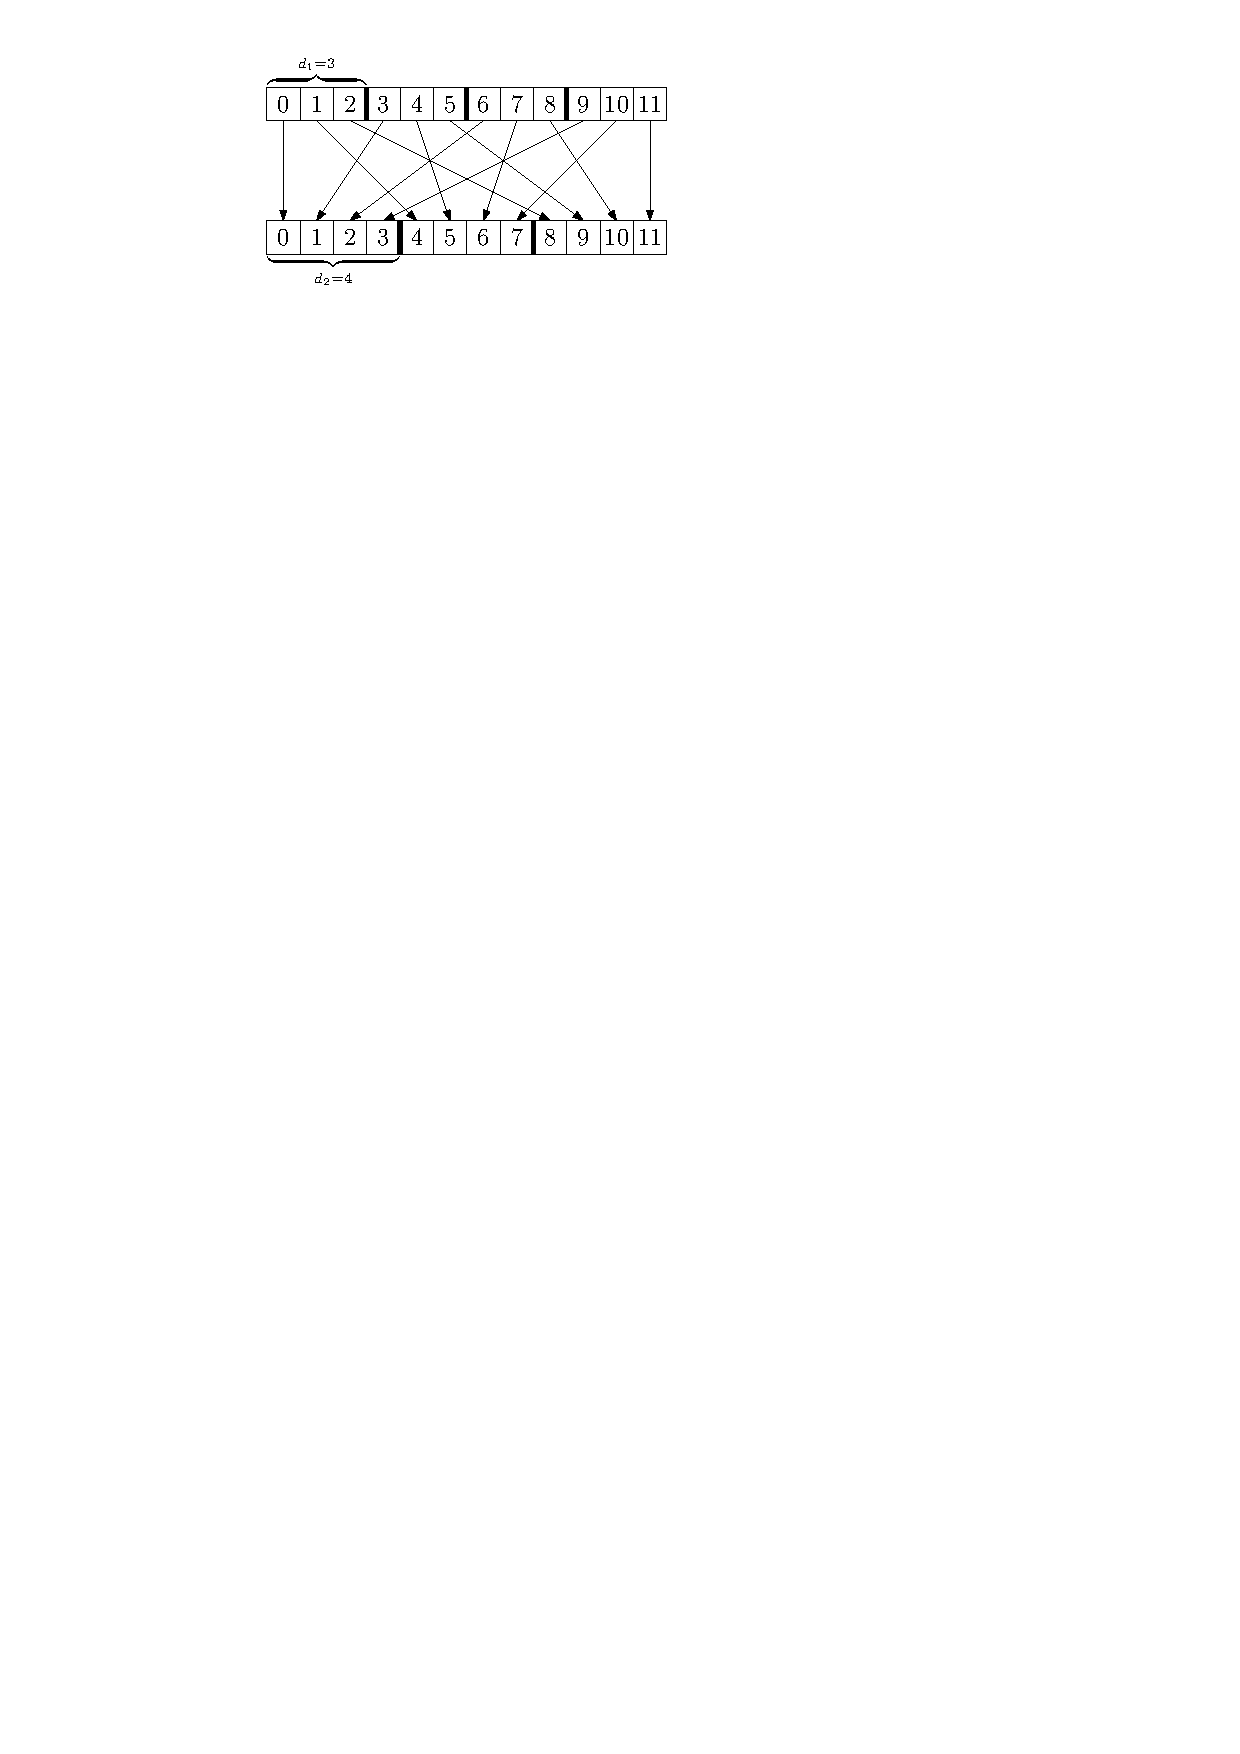
\includegraphics{transpose}
\caption{Illustration of the \texttt{transpose} operation}
\label{fig:transpose}
\end{figure}

\section{Evaluation}
\label{sec:evaluation}

\subsection{Setup}

We have tested the performance of FlowArrays in comparison with
ParArrays by calculating the scalar product of two vectors. Refer to
fig~\ref{fig:scalar-product} for the implementation of the
benchmark. You'll notice the operations \texttt{zipMap} and
\texttt{zipMapFold}: These are consolidated operations that use the
\texttt{FAJob} structure but do not store intermediate results. As we
will see they greatly increase performance.

\begin{figure}
\begin{minipage}[t]{6cm}
\begin{alltt}
{\scriptsize
val x = FlowArray.tabulate(size)(x => x*x)
val y = FlowArray.tabulate(size)(x => x*x)

(x zip y).map(x => x._1 * x._2).fold(0)(_ + _).blocking
// OR
(x zipMap y)(_ * _).fold(0)(_ + _).blocking
// OR
(x zipMapFold y)(_ * _)(0)(_ + _).blocking
}
\end{alltt}
\end{minipage}
\caption{Implementation of scalar product with FlowArrays}
\label{fig:scalar-product}
\end{figure}

We have varied the size of the two vectors from $8 \cdot 10^6$ to $13
\cdot 10^6$ elements with full parallelization. Further, we have
tested the scalability by setting the parallelism level to $1,2$ and
$4$ for FlowArrays (ParArrays have only been measured with full
parallelism). The metrics we collected were the execution time and the
garbage collection time.

The benchmarks have been executed on a Intel i7-2620M with a java
version 1.7.0\_04, Java(TM) SE Runtime Environment (build
1.7.0\_04-b20), Java HotSpot(TM) 64-Bit Server VM (build 23.0-b21,
mixed mode).

\subsection{Results}

Please refer to figs~\ref{fig:par-bench},\ref{fig:size-bench} for the
results of the benchmarks. In both figures, we show the total
execution time, the time spent in garbage collection and the
``normalised execution time'', i.e. the total time minus the time
spent in garbage collection. Please note that the GC time is an
approximation and hence the ``normalised execution time'' may become
negative.

\begin{figure}
\subfigure[Execution Time]{\plot{par-time}}
\subfigure[GC Time]{\plot{par-gctime}}
\subfigure[Normalised Time]{\plot{par-ntime}}
\caption{Parallelization benchmarks of scalar product}
\label{fig:par-bench}
\end{figure}

\begin{figure}
\subfigure[Execution Time]{\plot{size-time}}
\subfigure[GC Time]{\plot{size-gctime}}
\subfigure[Normalised Time]{\plot{size-ntime}}
\caption{Size benchmarks of scalar product}
\label{fig:size-bench}
\end{figure}

\subsection{Interpretation}
First of all we must notice the huge overhead that garbage collection
brings, especially for the benchmark using the simple \texttt{zip},
\texttt{map} and \texttt{fold} operations, against which --
unfortunately -- the actual calculation time becomes negligible. Note
that octave \cite{octave} takes around $290 ms$ for the same
calculation on the same machine, we can hence say the execution times
(when disregarding garbage collection) are comparable.

Other benchmarks for matrix multiplication that have been mostly
written but not yet been brought to a conclusion have already
indicated that garbage collection might take a big amount of time
during calculation.

We must come to the unfortunate conclusion, that allocating and
storing small intermediate steps seems to be a severe performance
killer. When continuing in the flow approach, means of reducing
intermediate storage steps might need to be considered such as the
\texttt{zipMap} and the \texttt{zipMapFold} operations that have
greatly increased performance.

\section{Conclusion}
\label{sec:conclusion}
TODO write properly
\begin{enumerate}
\item We have implemented fixed-size FlowArrays and handled most
  challenges.
\item Benchmarks suggest garbage collection due to full intermediate
  result storage is a performance issue
\item Consolidated operations such as \texttt{zipMap} /
  \texttt{zipMapFold} can greatly improve performance.
\item A way to automate the conversion / reduction zip, map $\to$
  zipMap would be great.
\end{enumerate}

\bibliographystyle{abbrv}
\bibliography{bib}

\end{document}

%%% Local Variables: 
%%% mode: latex
%%% TeX-master: t
%%% End: 
